\documentclass[halfparskip]{scrartcl}

\title{Arduino-Ampel}
\subtitle{Dokumentation}
\author{Heye Hamadmad}
\date{\today{}, Bremen}

\usepackage{ucs}
\usepackage[utf8x]{inputenc}
\usepackage[T1]{fontenc}

\usepackage[ngerman]{babel}

\usepackage{graphicx} 

\usepackage{hyperref}

\usepackage{listings}

\lstdefinestyle{customc}{
  breaklines=true,
  language=C,
}

\begin{document}
\maketitle

\textit{Diese Dokumentation wurde entnommen von \url{http://github.com/hamadmad/arduino-ampel/}}

Das Projekt dient zur Demonstration einer kleinen Ampelschaltung und ist ggf. zur Realisierung eines Modellbauprojekts geeignet.

Die Hardware entspricht einem Shield für einen Arduino UNO und ist dementsprechend auch mit einem Arduino Duemilanove kompatibel.
Eingesetzt werden 5 LEDs um die Lampen der Ampel zu symbolisieren, sowie ein Taster zum Betätigen der Fußgängerampel.
Außerdem existiert ein Port zur Seriellen Kommunikation über z.B. ein Bluetooth-Modul mit einer zentralen Steuereinheit oder zur Meshartigen Vernetzung und Selbstorganisation mit anderen Ampeln.

Die Software basiert ausschließlich auf einer rudimentären state-machine. Funktionen zur Kommunikation mit anderen Plattformen sind \textbf{NICHT} implementiert. Da unter Umständen die PWM-Pins eingesetzt werden können, die nicht auf dem Arduino Duemilanove vorhanden sind, ist dieser softwareseitig \textbf{NICHT} unbedingt unterstützt.

\section{Hardware}
\label{sec:hardware}
Die Hardware orientiert sich am folgenden Schaltplan:
\begin{center}
    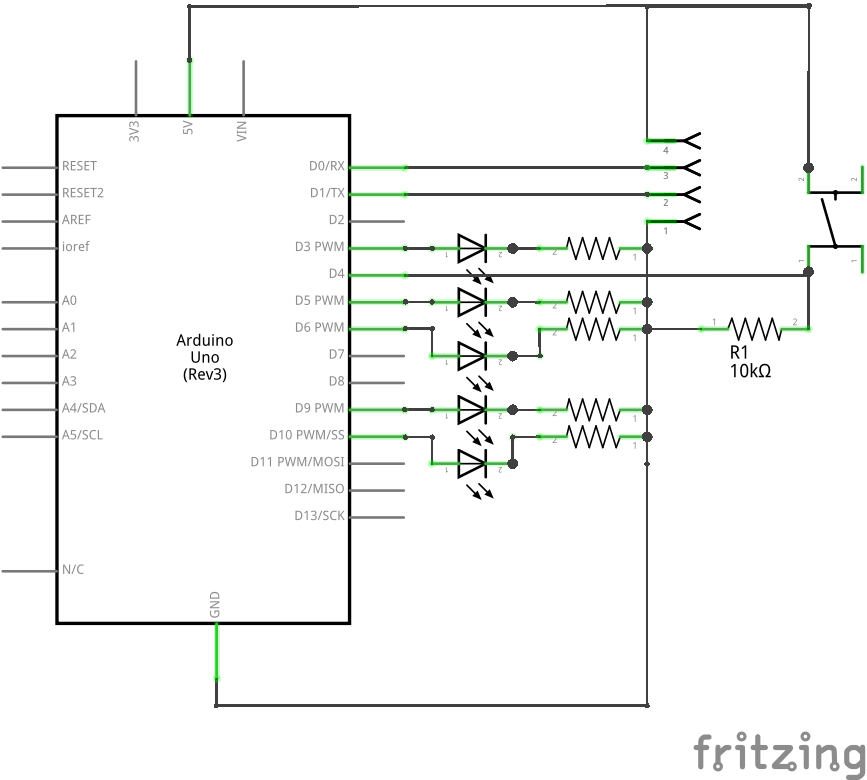
\includegraphics[width=1\textwidth]{hardware/schaltplan}
\end{center}
Die LEDs werden jeweils mit einem 150Ohm Widerstand an Masse geführt.
Der Taster wird mit einem 10kOhm Pull-Down-Widerstand ebenfalls an Masse geführt.
Der Steckverbinder wird außer an die beiden Pins zur Seriellen Kommunikation auch mit den Stromleitungen verbunden um ggf. ein Erweiterungsboard mit Strom versorgen zu können. Bei Zukünftigen Versionen könnte außerdem über eine I2C oder OneWire Verbindung nachgedacht werden.

Die folgenden Teile werden benötigt:
\begin{itemize}
    \item 1	Arduino Uno Rev3 / Duemilanove
    \item 4   [OPTIONAL] Buchsenleiste (J1)
    \item 2	LED Rot (LED1, LED4)
    \item 2	LED Grün (LED2, LED5)
    \item 1	LED Gelb (LED 3)
    \item 1	10k$\Omega$ Widerstand (R1)
    \item 5	150$\Omega$ Widerstand (R2-6)
    \item 1	Taster (S1)
\end{itemize}

Das Shield kann nach dem folgenden Layout aufgebaut werden:
\begin{center}
    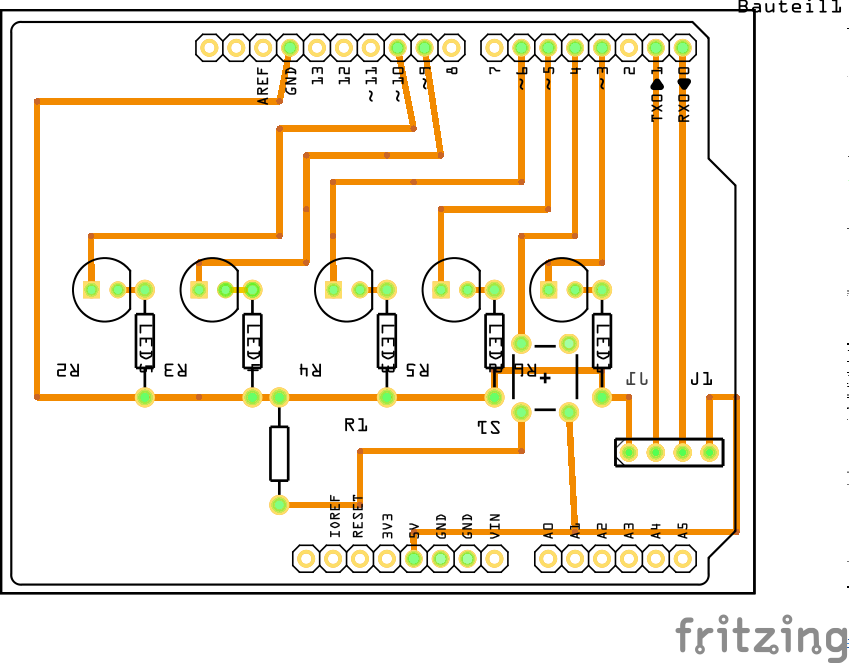
\includegraphics[width=1\textwidth]{hardware/board}
\end{center}
Die Dateien zum Anfertigen von Platinen finden sich im Unterordner hardware/board\_pdf

Es ist darauf zu achten, dass statt der vorgeschlagenen LEDs und Taster auch Verlängerungskabel angebracht werden können um die eigentliche Ampelanlage klein zu halten. Des Weiteren ist die Buchsenleiste optional. 

\section{Software}
\label{sec:software}
Der Quellcode findet sich hier und außerdem im Unterverzeichnis code/code

\lstinputlisting[style=customc]{code/code/code.ino}

Der Quellcode besteht hauptsächlich aus einer state-machine in der der Ablauf der Ampelphasen definiert ist.
Der Timer benötigt die Bibliothek TimerOne.
Es existieren die folgenden optionalen Konfigurationsmöglichkeiten:

\begin{itemize}
    \item UseRY Entscheidet darüber, ob die Gelbe Leuchte am Ende der Rotphase signalisieren soll, dass es gleich weitergeht. Standardmäßig aktiviert.
    \item AutomaticPedestrianPhase ermöglicht die automatische Unterbrechung der Grünphase für die Autofahrer ohne die Anfrage eines Fußgängers. Standardmäßig deaktiviert.
\end{itemize}

Die Zeiten für die Phasen können ebenfalls durch das Anpassen der dafür zuständigen defines geändert werden.

\section{Inbetriebnahme}
\label{sec:inbetriebnahme}
Ggf. müssen die Zeiten für die Ampelphasen noch im Code angepasst werden.
Sobald eine Stromzufuhr vorhanden ist, läuft die Ampel autonom. Die Funktion zur Kommunikation unter Benutzung der seriellen Schnittstelle ist noch nicht implementiert.

\section{Weiterhin zu beachten:}
\label{sec:weiterhin}
Der gesamte Quellcode wurde nicht getestet. Er sollte sich zwar kompilieren lassen, aber die Funktionsfähigkeit kann nicht garantiert werden.
\end{document}
